\documentclass[a4paper, 12pt]{article}

\usepackage[T2A]{fontenc}
\usepackage[utf8]{inputenc}
\usepackage[english,russian]{babel}
\usepackage[left=15mm, top=20mm, right=15mm, bottom=20mm, nohead, nofoot]{geometry}

\usepackage{hyperref}
\usepackage{graphicx}
\usepackage{wrapfig}
\usepackage{afterpage}
\usepackage{amsmath, amsfonts, amssymb, amsthm, mathtools}
\author{Хомутов Андрей, группа Б06-903}
\title{ВПВ по курсу "Электричество и магнетизм" \\ Конденсатор на высоких частотах}
\date{22 декабря 2020 г.}
%%%%%%%%%%%%%%%%%%%%%%%%%%%%%%%%%%%%%%%%%%%%%%%%%%%%%%%%%%%%%%%%%%%%%%%%%
\usepackage{graphicx, wrapfig, subcaption, setspace, booktabs}
\usepackage[protrusion=true, expansion=true]{microtype}
\usepackage[english]{babel}
\usepackage{sectsty}
\usepackage{url, lipsum}
\newcommand{\HRule}[1]{\rule{\linewidth}{#1}}
\onehalfspacing
\setcounter{tocdepth}{5}
\setcounter{secnumdepth}{5}
%%%%%%%%%%%%%%%%%%%%%%%%%%%%%%%%%%%%%%%%%%%%%%%%%%%%%%%%%%%%%%%%%%%%%%%%%


\begin{document}

\title{ \normalsize \textsc{Лабораторная работа по физической химии}
		\\ [4.0cm]
		\HRule{0.5pt} \\ [0.3cm]
		\LARGE \textbf{{Кинетика обесцвечивания красителя}}
		\HRule{0.5pt} \\ [0.1cm]
		\normalsize  \vspace*{18\baselineskip}}

\date{}

\author{Шамарина Екатерина, Б06-903 \\
		Хомутов Андрей, Б06-903 \\
ФБМФ, 2021\\ }

\maketitle
\thispagestyle{empty}
\newpage
%%%%%%%%%%%%%%%%%%%%%%%%%%%%%%%%%%%%%%%%%%%%%%%%%%%%%%%%%%%%%%%%%%%%%%%%%
\section*{Цель работы} 
Определить  порядок  реакции  по  красителю(метиловый фиолетовый)  и  по NaOH, на основе  полученных  измерений  рассчитать  константу  скорости  реакции.Исследовать влияние ионной силы раствора на скорость реакции.
%%%%%%%%%%%%%%%%%%%%%%%%%%%%%%%%%%%%%%%%%%%%%%%%%%%%%%%%%%%%%%%%%%%%%%%%%
 
\section{Теоретическая часть}
\subsection{Измерения спектрофотометром}
\textbf{Закон светопоглощения Бугера-Ламберта-Бера}:
\begin{equation}
D = lg\frac{I}{I_{0}} = \varepsilon_{\lambda}Cl,
\end{equation}
где D -- оптическая плотность; $I_{0}$-- интенсивность падающего света; I -- интенсивность
света, прошедшего через образец; C -- концентрация вещества; l -- толщина
поглощающего слоя; $\varepsilon_{\lambda}$ -- коэффициент молярной экстинкции при длине волны $\lambda$ (здесь совпадает с коэффициентом поглощения, но в общем случае
учитывается также процесс ослабления света из-за рассеяния $\varepsilon_{\lambda} = \varepsilon_{\lambda,abs} + \varepsilon_{\lambda,scatt}$ ).\\
Для реакции первого или псевдопервого порядка константа скорости:
\begin{equation}
k_{1} = \frac{1}{t} \cdot \ln \frac{C_{0}}{C(t)} = \frac{1}{t} \cdot \ln \frac{D_{0}}{D(t)},
\end{equation}
где $D_{0}$ -- начальная величина оптической плотности, $D(t)$ -- ее значение к моменту времени t.
\subsection{Влияние среды на скорость ионных реакций}
Реакции между заряженными частицами в растворах зависят от ионной силы J:
\begin{equation}
J = \frac{1}{2} \sum_i^n C_{i} Z_{i}^{2},
\end{equation}
где  $C_{i}$ и $Z_{i}$ -- концентрации и заряды различных ионов.\\
В теории переходного состояния или активированного комплекса скорость
химической реакции:
\begin{equation}
W = (k_{\text{Б}}T/h)\cdot C^{\#}
\end{equation}
где Т -- температура, $k_{\text{Б}}$ и h -- константы Больцмана и Планка, а $C^{\#}$ -- концентрация активированного комплекса. Множитель $k_{\text{Б}}T/h$ -- не зависящая от природы реагентов частота перехода комплексов через вершину активационного барьера.\\
Так как в данной теории постулируется существование равновесия между
исходными реагентами и активированным комплексом, концентрацию последнего
получаем, используя расчет констант
равновесия $K_{a}^{\#}$. Для бимолекулярной реакции с участием заряженных частиц A и B в растворе:
\begin{equation}
K_{a}^{\#} = (a^{\#}/a_{A}a_{B}) = (C^{\#}/C_{A}C_{B})\cdot (f^{\#}/f_{A}f_{B}),
\end{equation}
a и f -- активности и коэффициенты активности реагентов
и активированного комплекса $(a_{i} = f_{i}C_{i})$, его концентрация:
\begin{equation}
C^{\#} = K_{a}^{\#}(f_{A}f_{B}/f^{\#})C_{A}C_{B},
\end{equation}
Выражение для константы скорости реакции:
\begin{equation}
k = W/(C_{A}C_{B}) = (k_{\text{Б}}T/h)K_{a}^{\#}(f_{A}f_{B}/f^{\#}) = k_{0}(f_{A}f_{B}/f^{\#}),
\end{equation}
где в $k_{0}$ включены все независимые от свойств среды параметры.
Коэффициенты активности ионов в теории сильных электролитов
Дебая-Хюккеля:
\begin{equation}
-\lg f_{i} = 1,823\cdot 10^{6} (\varepsilon \cdot T)^{-3/2}Z_{i}^{2}J^{1/2}
\end{equation}
для воды $(\varepsilon = 78,25)$ при Т = 298 К:
\begin{equation}
-\lg f_{i} \cong 0,51 Z_{i}^{2}J^{1/2}
\end{equation}
С учетом $Z^{\#} = Z_{A} + Z_{B}$:
\begin{equation}
\lg \frac{k}{k_{0}} \cong 1,02 Z_{A}Z_{B}J^{1/2}
\end{equation}


\subsection{Кинетика обесцвечивания фенолфталеина}
\begin{figure}[h!]
    \begin{center}
    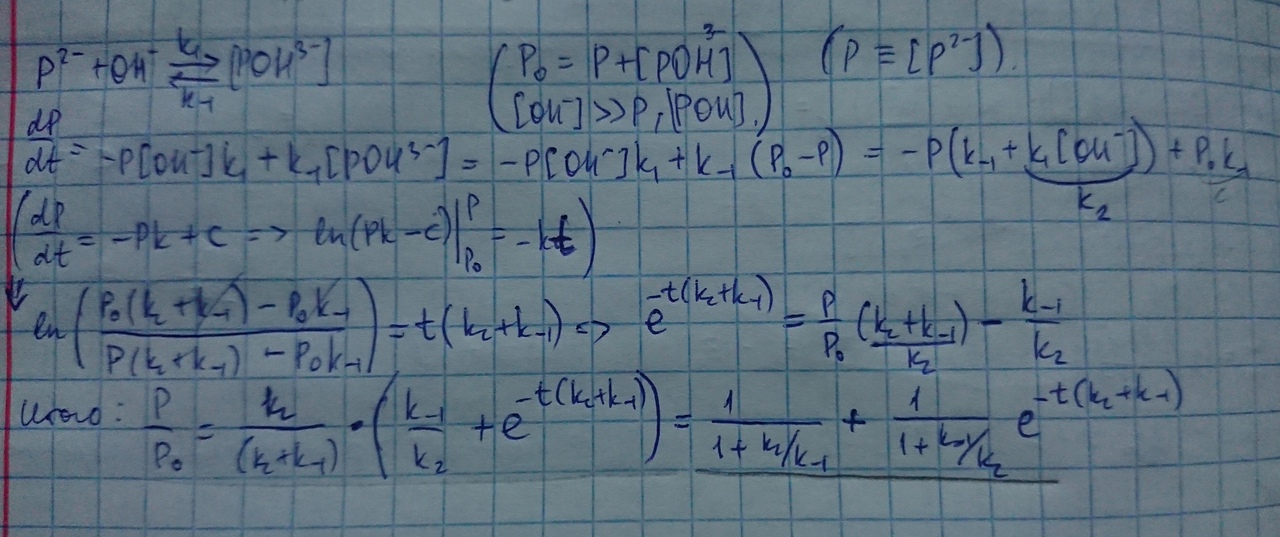
\includegraphics[width=1\textwidth]{вывод.jpg}
    \end{center}
\end{figure}
\newpage


\section{Практическая часть}

\subsection{Снятие спектра поглощения метилового фиолетового}
Измерив зависимость оптической плотности от длины волны, находим что максимум поглощения наблюдается при $\lambda$ = 576 нм, на ней и будут проведены последующие измерения.
 \begin{figure}[h!]
    \begin{center}
    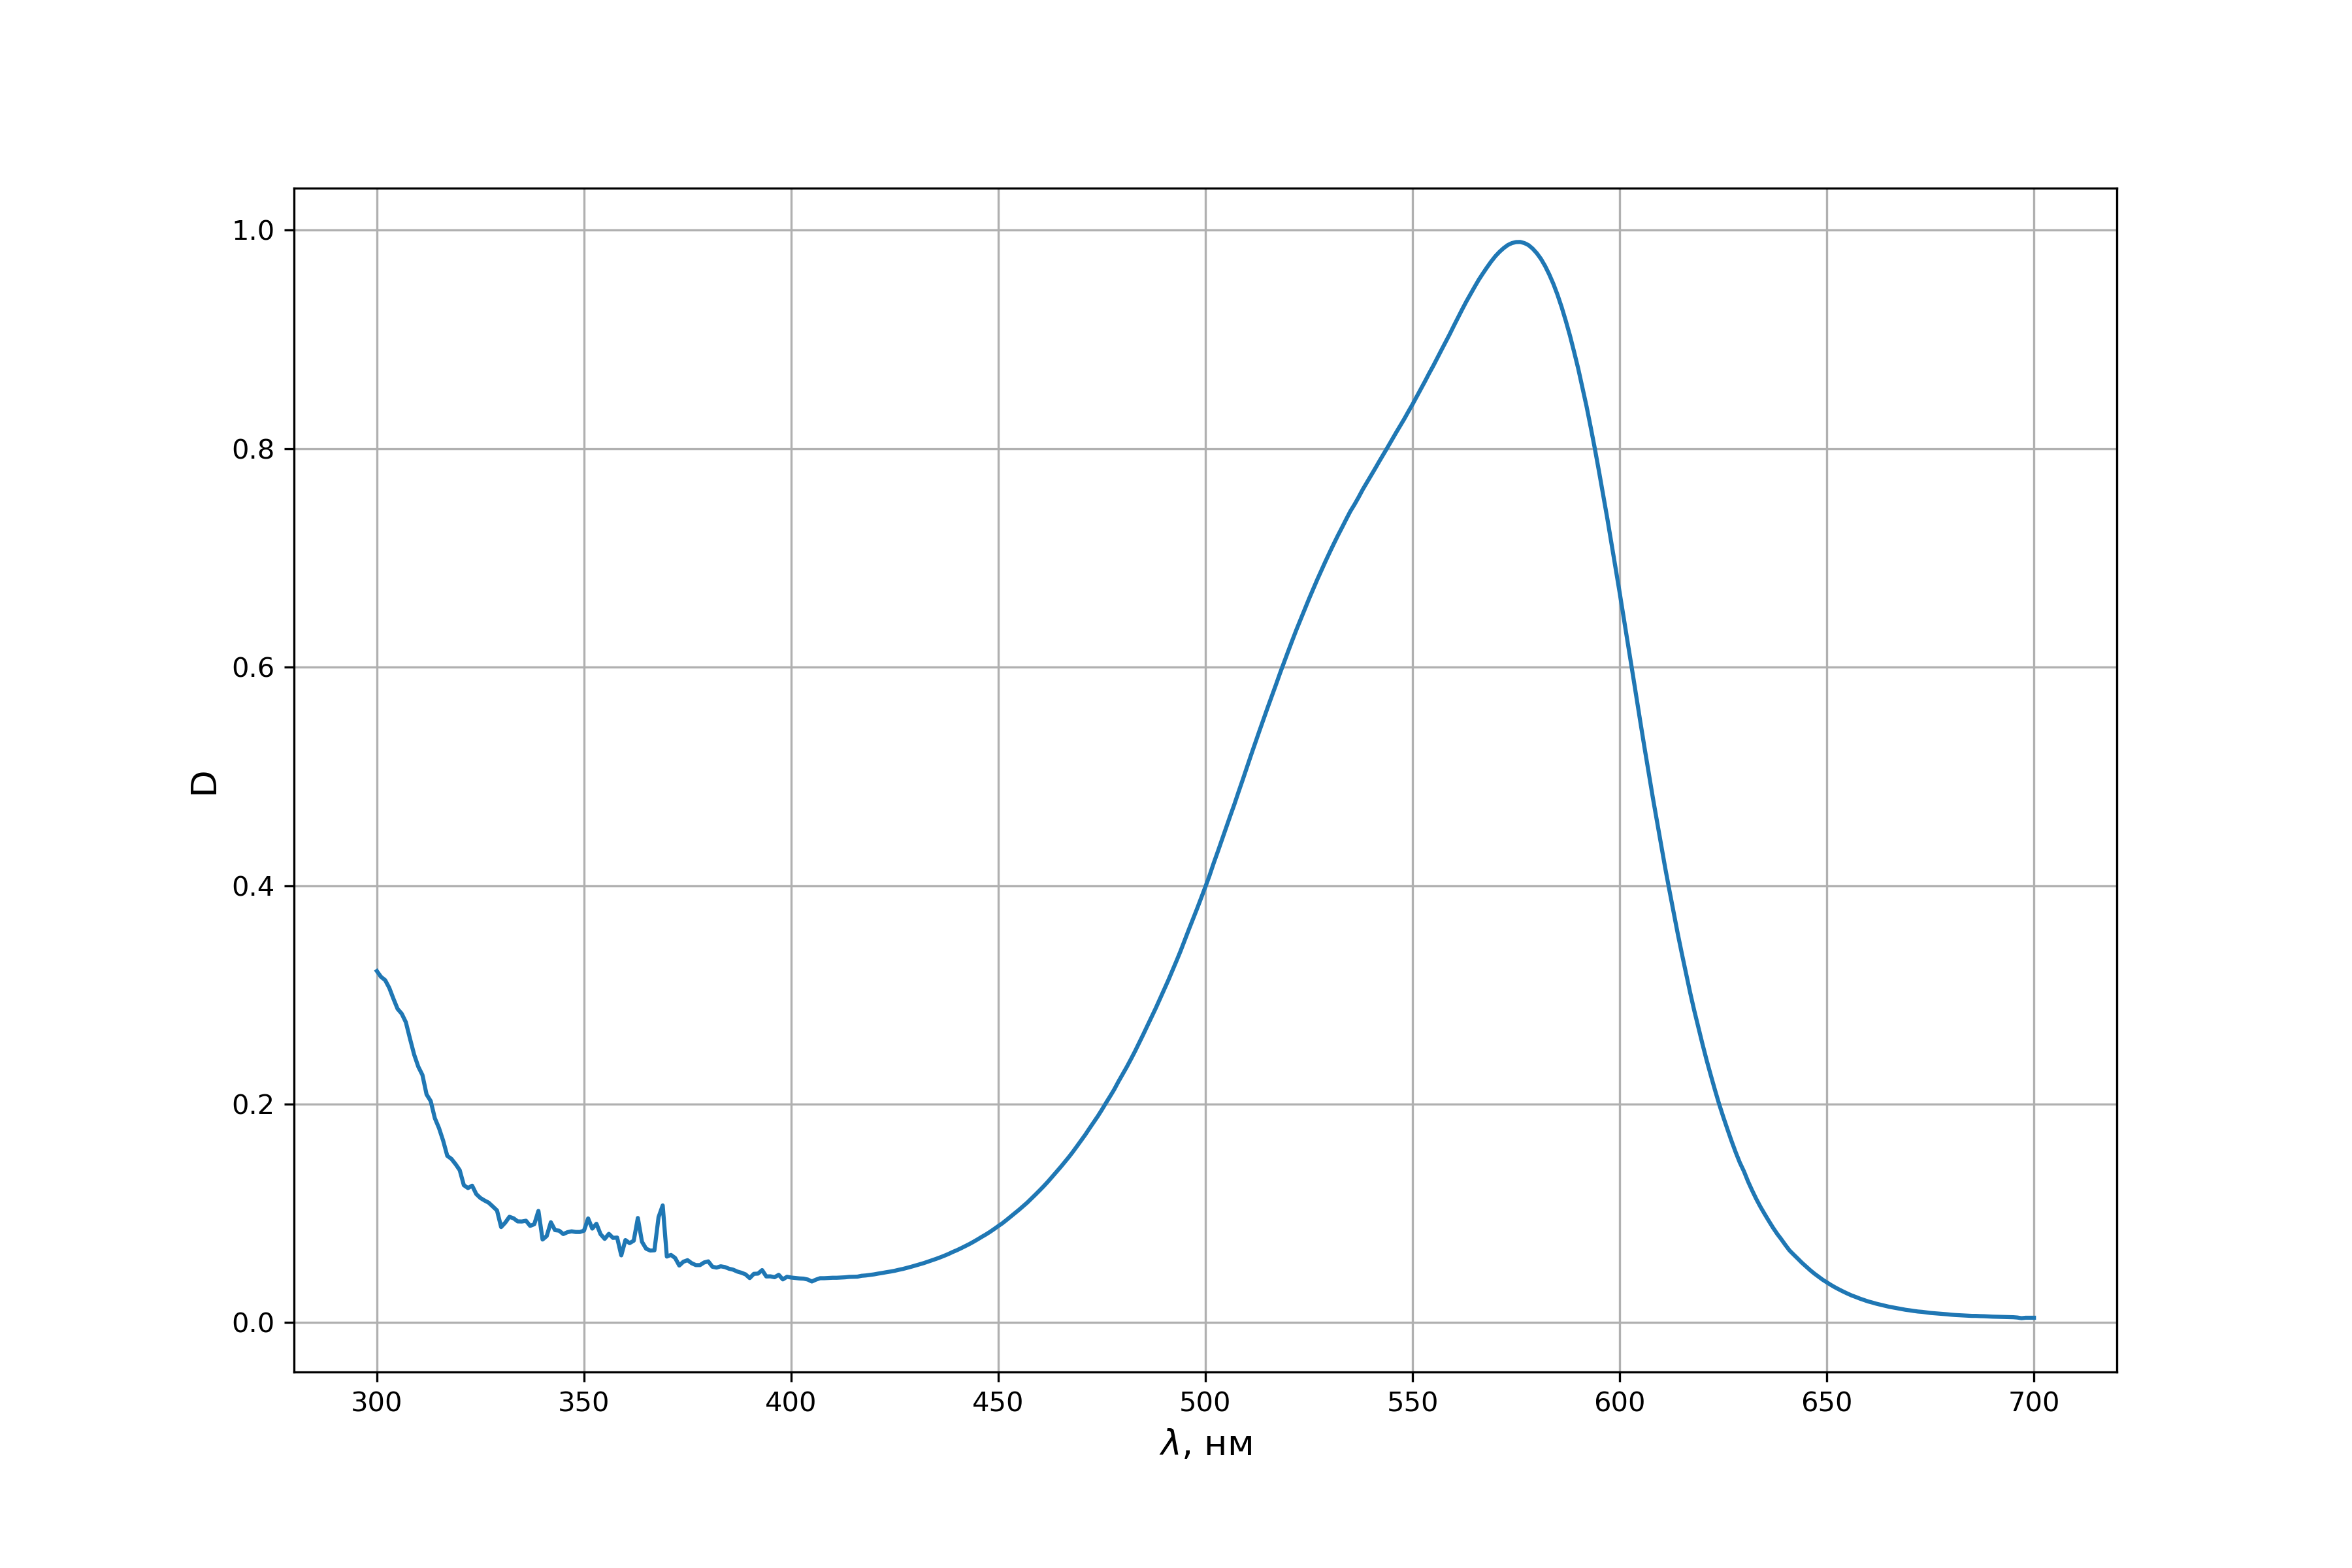
\includegraphics[width=1\textwidth]{fig1.png}
    \end{center}
    \caption{Спектр поглощения метилового фиолетового}
\end{figure}

%%%%%%%%%%%%%%%%%%%%%%%%%%%%%%%%%%%%%%%%%%%%%%%%%%%%%%%%%%%%%%%%%%%%%%%%%
\subsection{Исследование зависимости скорости обесцвечивания от концентрации щелочи}

В этой серии экспериментов ионная сила раствора сохранялась постоянной и равной 0.1 М. На рис. 2 представлены кинетические кривые обесцвечивания красителя при различных концентрациях щелочи (серыми штриховыми линиями) и их аппроксимации функциями вида $\frac{D(t)}{D_0} = \frac{1}{1+k_2/k_{-1}} \cdot e^{-t(k_2+k_{-1})} + \frac{1}{1+k_{-1}/k_2}$ для учета того что устанавливается равновесие с продуктами реакции. В таблице 1 представлены расчетные константы скорости
 \begin{figure}[h!]
    \begin{center}
    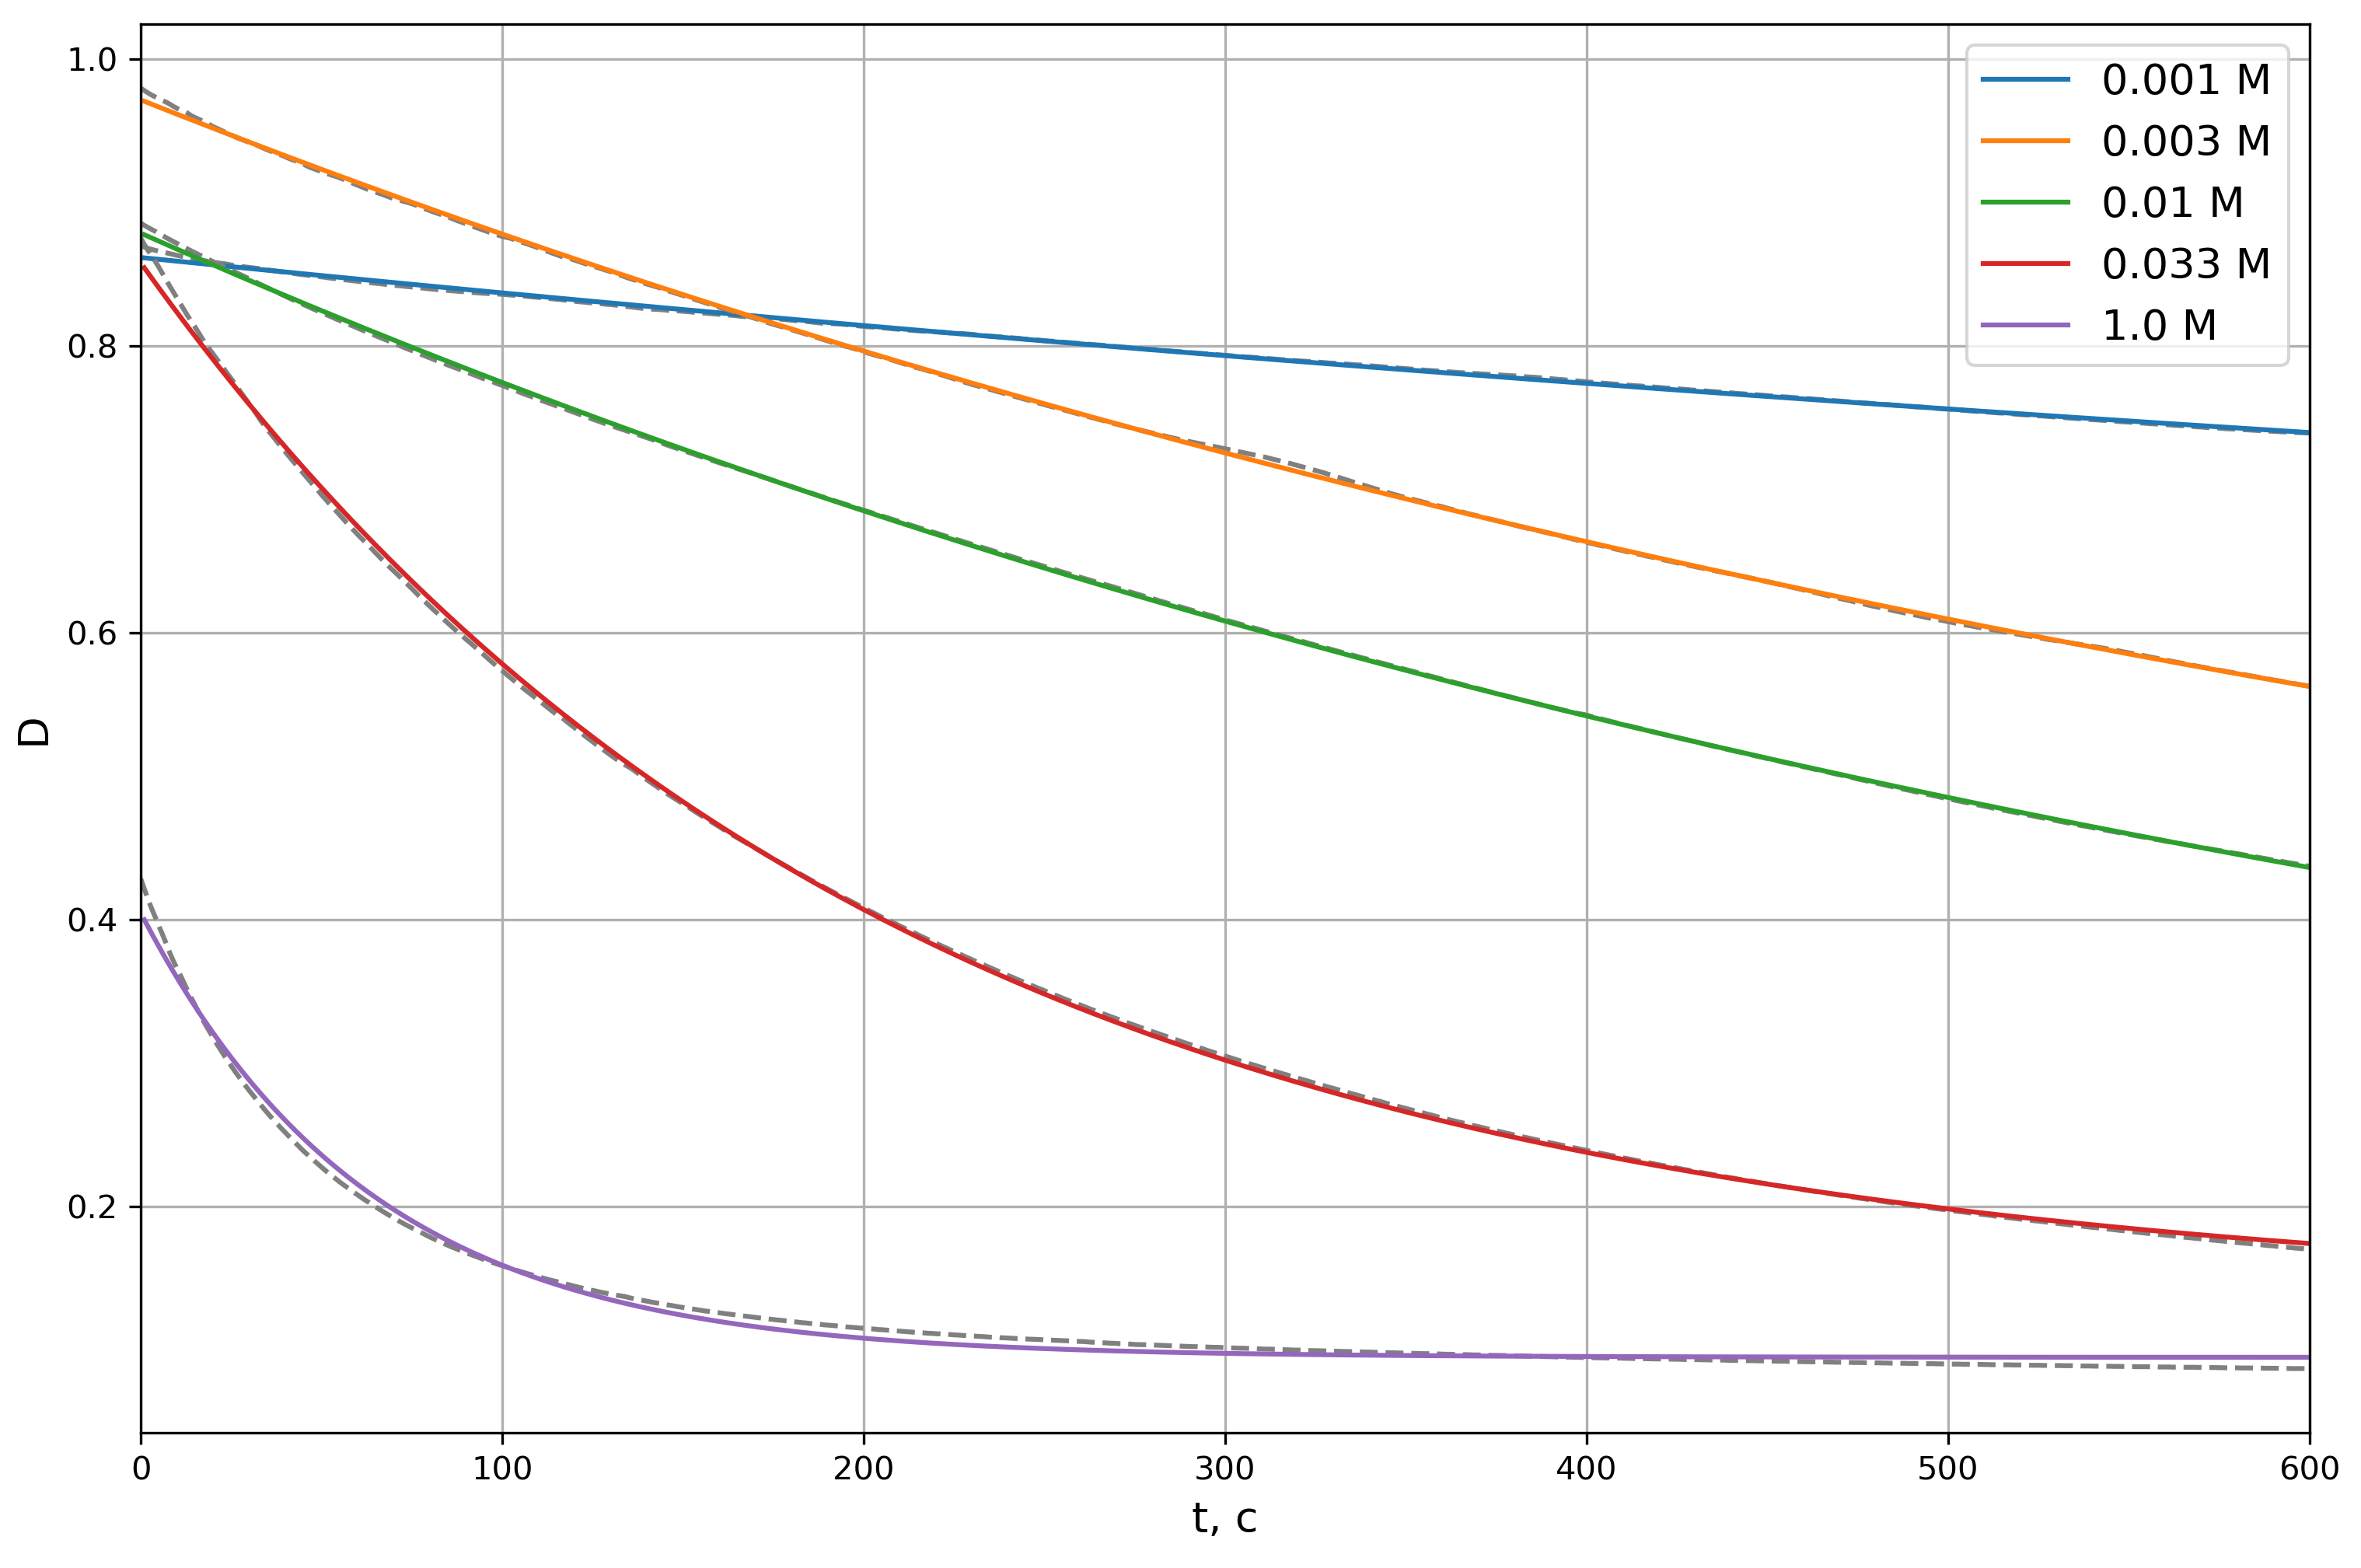
\includegraphics[width=0.9\textwidth]{fig2.png}
    \end{center}
    \caption{Кинетические кривые для различных концентраций щелочи с аппроксимацией}
\end{figure}

\begin{table}[h!]
\begin{center}
\caption{Константы скорости для различных концентраций щелочи}
\begin{tabular}{|l|c|c|c|c|c|}
\hline
C(NaOH), M               & 0,001 & 0,003 & 0,01  & 0,033 & 1     \\ \hline
$k_2, 10^{-3} c^{-1}$                       & 0,298 & 1,031 & 1,277 & 4,123 & 12,04 \\ \hline
$\delta k_2, 10^{-3} c^{-1}$  & 0,002 & 0,002 & 0,002 & 0,007 & 0,09  \\ \hline
\end{tabular}
\end{center}
\end{table}

\begin{figure}[h!]
    \begin{center}
    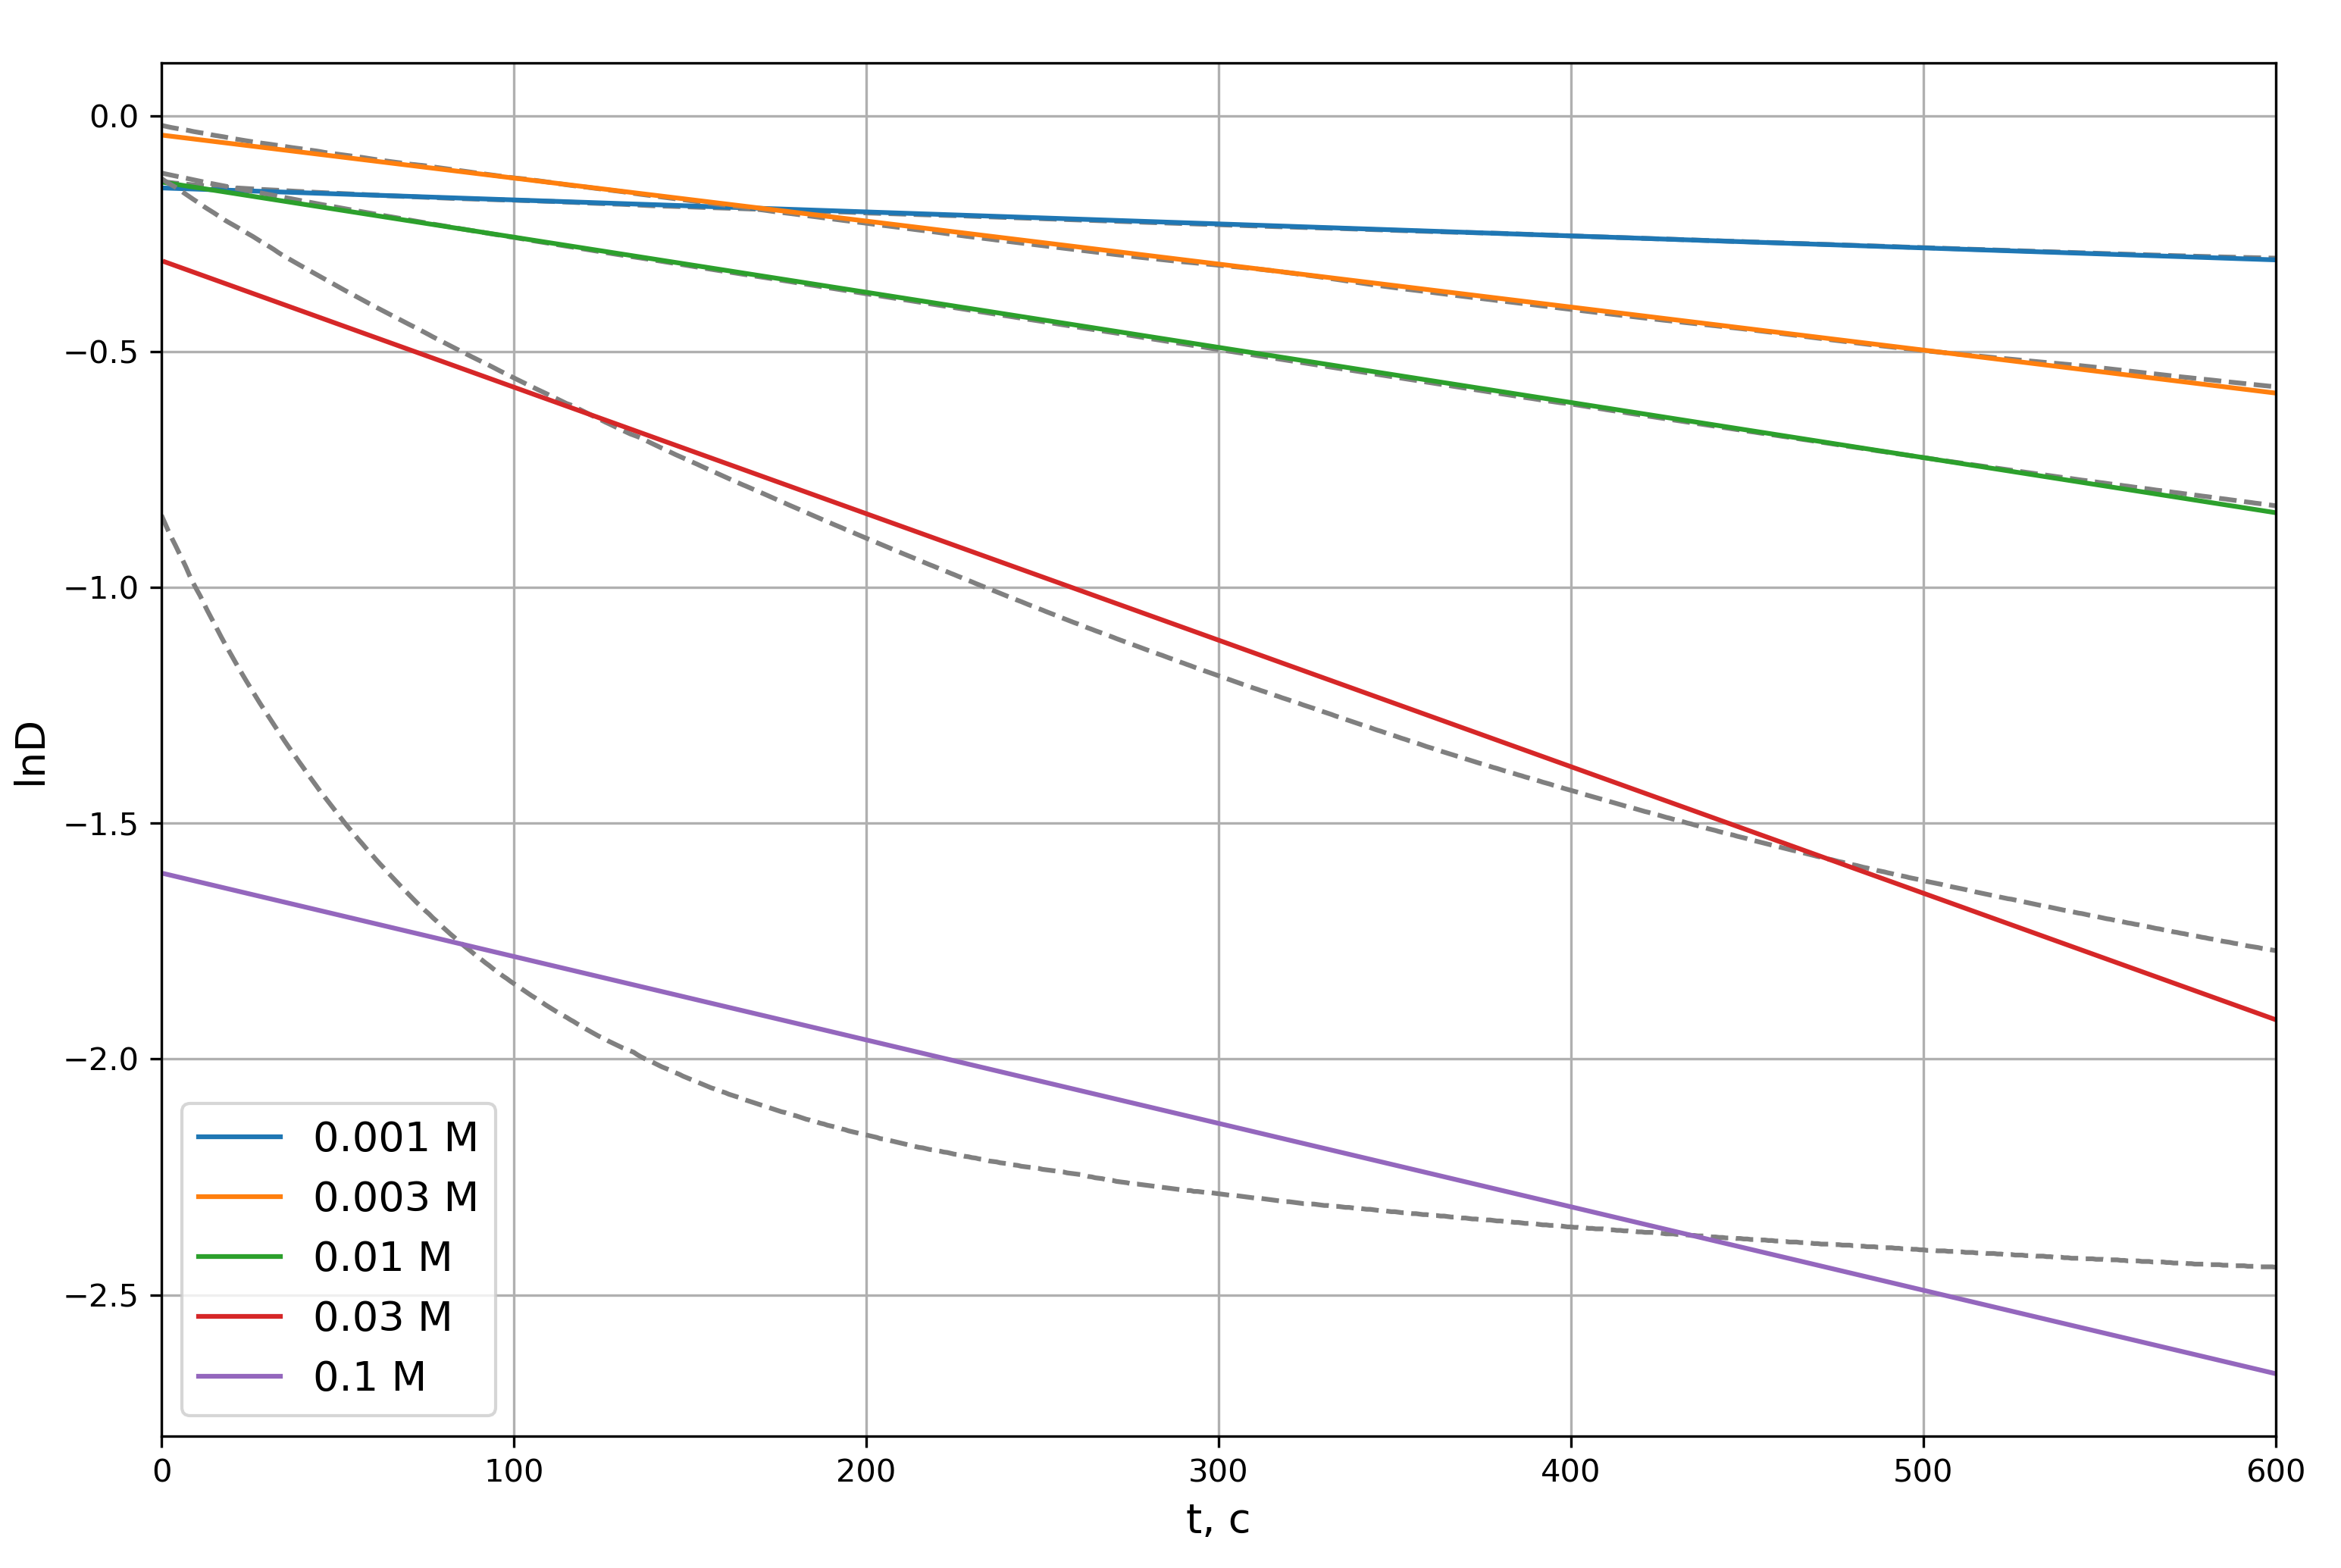
\includegraphics[width=0.9\textwidth]{1 lnD.png}
    \end{center}
    \caption{Линеаризация зависимости D(t) с аппроксимацией}
\end{figure}

Построив график lnD(t), убедимся, что реакция имеет (псевдо)первый порядок по красителю, по крайней мере при небольших концентрациях NaOH.

Порядок реакции m по $OH^-$ и константу реакции $k_1$ можно определить, вспомнив, что $k_2 = k_1 \cdot [OH^-]^m$, то есть $ln k_2 = ln k_1 + m \cdot ln([OH^-])$, и построив график в соответствующих координатах. Из-за того, что часть опытов происходила с неисправной пипеткой, на Рис.4 проведём две прямые, предположительно описывающие зависимость $ln k_2 (ln([OH^-]))$. m получились 1.09 и 0.97, что подтверждает предположение о первом порядке реакции по щёлочи. $ln k_1$ из графиков: -1.110 и -2.122. Среднее: $ln k_1 = -1.6 \pm 0.5 \Rightarrow k_1 = (0.20\pm 0.10) \frac{1}{c \cdot M}$

\begin{figure}[h!]
    \begin{center}
    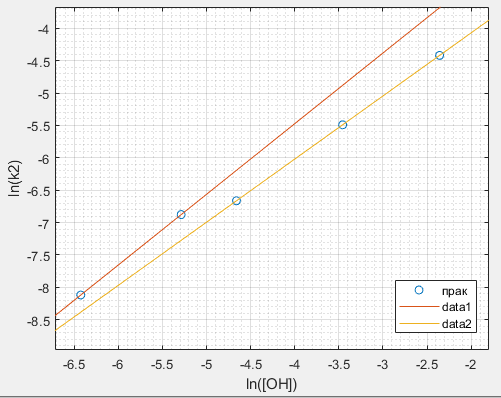
\includegraphics[width=0.7\textwidth]{1 lnK2(lnC).png}
    \end{center}
    \caption{Линеаризация зависимости $k_2([OH^-])$ }
\end{figure}


\newpage
%%%%%%%%%%%%%%%%%%%%%%%%%%%%%%%%%%%%%%%%%%%%%%%%%%%%%%%%%%%%%%%%%%%%%%%%%
\subsection{Исследование зависимости скорости обесцвечивания от ионной силы}


В этой серии измерений концентрация NaOH оставалась равной 0.01 М и варьировалась ионная сила раствора с помощью NaCl от 0.01 до 1 М. 

Зависимости были аппроксимированы функциями вида $D = D_0 e^{-kt}( +const)$ (без и с константой соответственно). В таблице представленны вычисленные константы скорости реакций псевдопервого порядка для обоих вариантов.
 \begin{figure}[h!]
    \begin{center}
    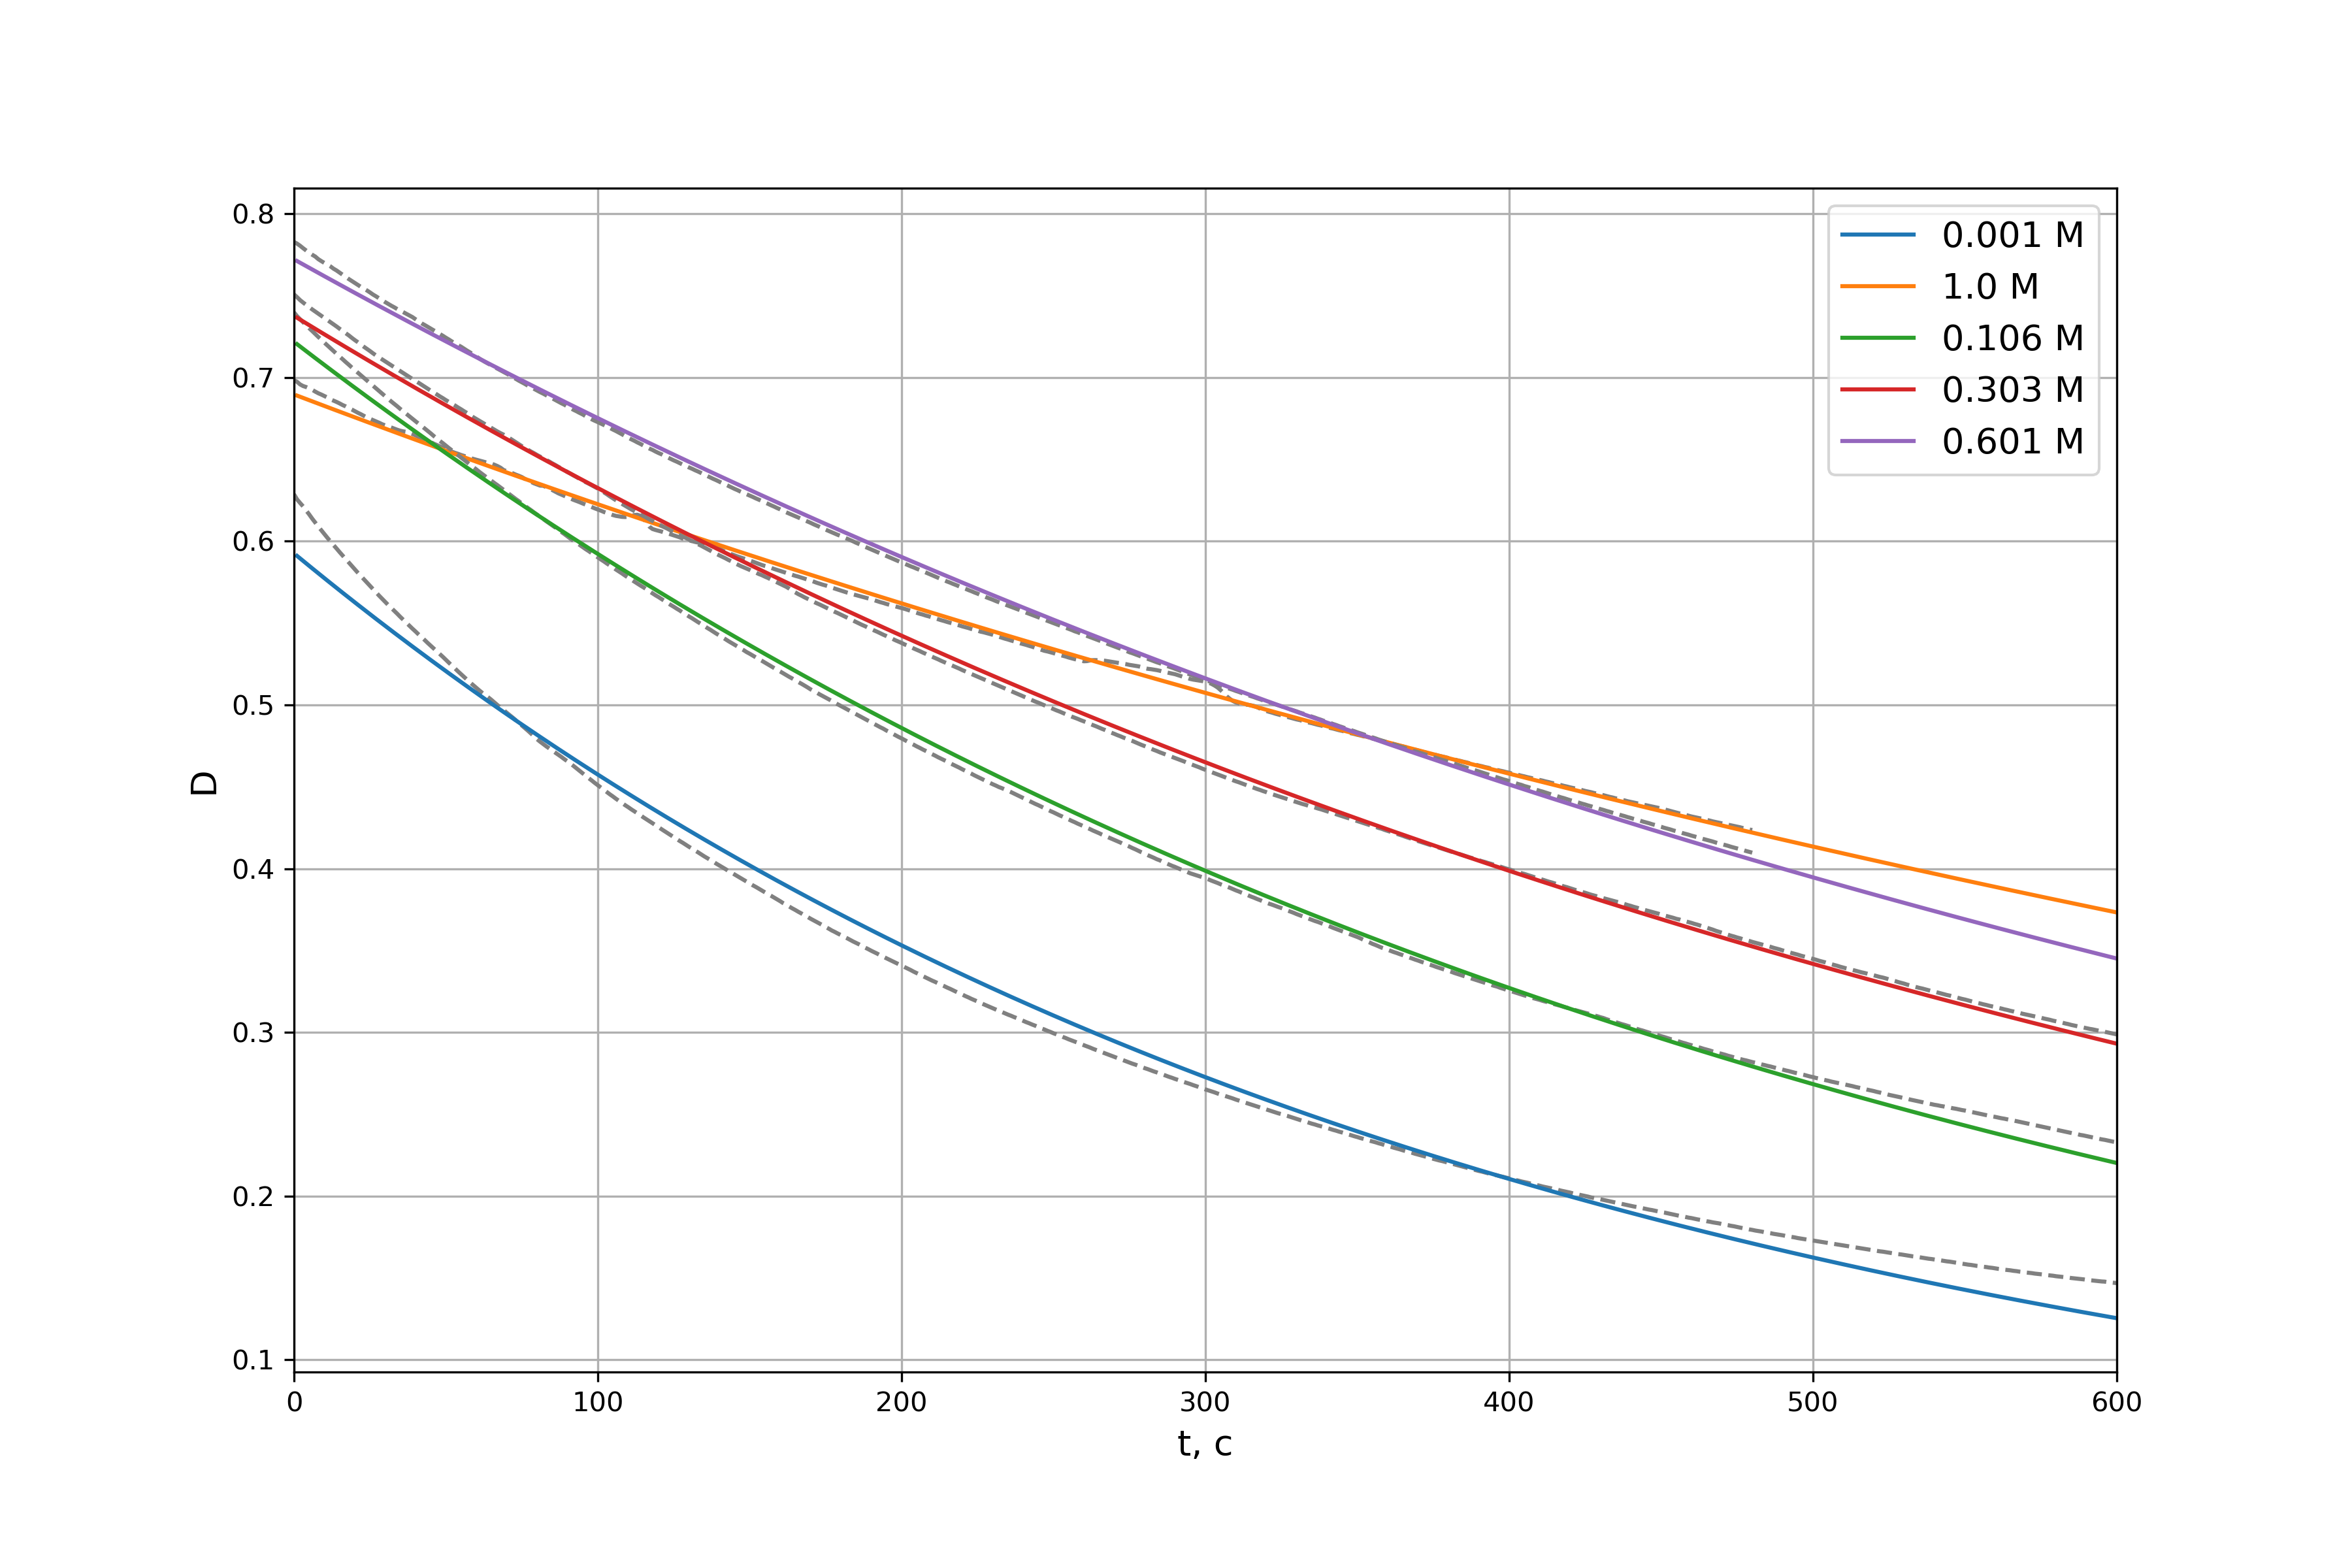
\includegraphics[width=1\textwidth]{fig3.2.png}
    \end{center}
    \caption{Кинетические кривые для различных ионных сил с аппроксимацией}
\end{figure}

\begin{table}[h!]
\begin{center}
\caption{Константы скорости для различных ионных сил}
\begin{tabular}{|l|r|r|r|r|r|}
\hline
I, M                         & \multicolumn{1}{c|}{0,001} & \multicolumn{1}{c|}{0,106} & \multicolumn{1}{c|}{0,303} & \multicolumn{1}{c|}{0,601} & \multicolumn{1}{c|}{1} \\ \hline
$k, 10^3 c^{-1}$   & 2,59                       & 1,98                       & 1,54                       & 1,34                       & 1,02                   \\ \hline
$k_c, 10^3 c^{-1}$ & 3,77                       & 2,54                       & 1,91                       & 1,79                       & 1,35                   \\ \hline
\end{tabular}
\end{center}
\end{table}

Наклоны линейных аппроксимаций зависимостей логарифма констант от корня из ионной силы тоже совпадают. Получается $1.02 Z_A Z_{OH} \simeq -0.43 \pm 0.2$, откуда  $Z_A \simeq 0.42 \pm 0.2$

 \begin{figure}[h!]
    \begin{center}
    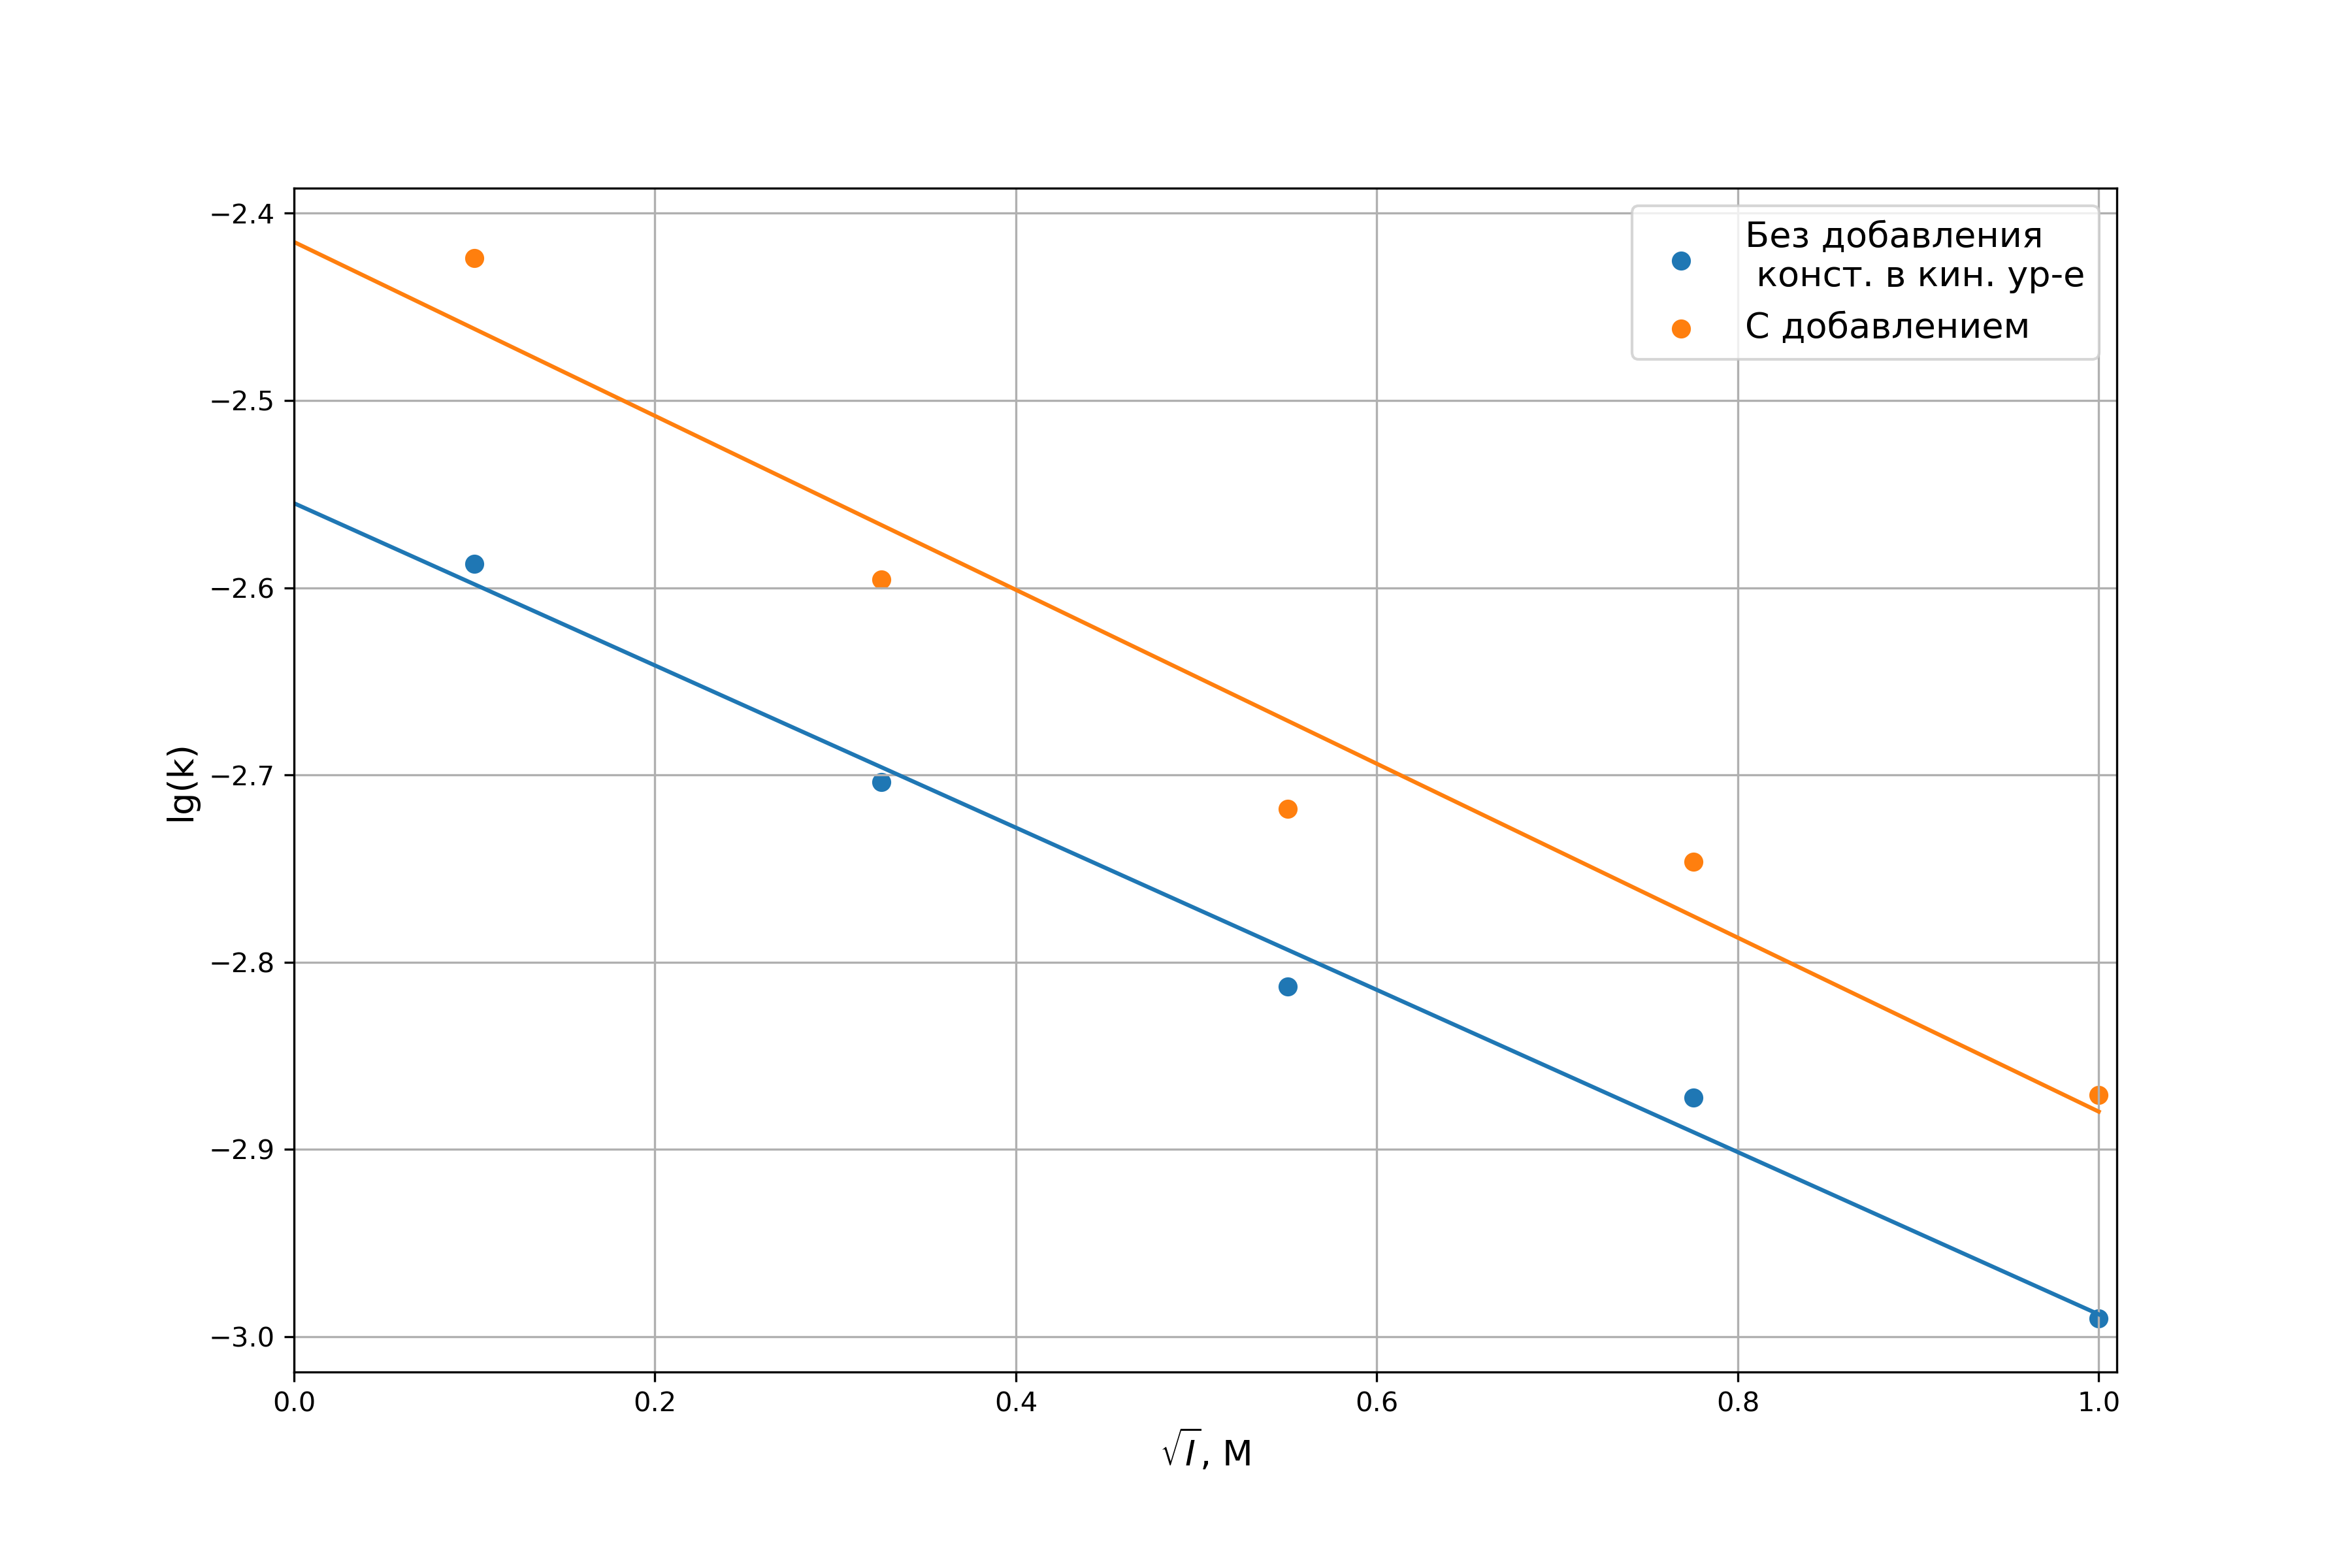
\includegraphics[width=1\textwidth]{fig3.3.png}
    \end{center}
    \caption{Зависимость $lgk(\sqrt I)$}
\end{figure}


\newpage
%%%%%%%%%%%%%%%%%%%%%%%%%%%%%%%%%%%%%%%%%%%%%%%%%%%%%%%%%%%%%%%%%%%%%%%%%
 \section{Выводы}
\begin{enumerate}
    \item С помощью спектрофотометра была изучена кинетика обесцвечивания красителя (метиловый фиолетовый). Определены порядки реакции по красителю и щёлочи. Рассчитана константа скорости реакции.
    \item Из кинетических кривых для различных ионных сил были определены константы, по зависимости которых от ионной силы было определено что солевой эффект заключается в падении скорости реакции с ростом ионной силы. То есть, краситель в реакции имеет положительный заряд

\end{enumerate}

\end{document}

\begin{table}[h!]
\begin{center}
\caption{...}
\begin{tabular}{|c|c|c|c|c|}

\end{tabular}
\end{center}
\end{table}


\begin{figure}[h!]
    \begin{center}
    \includegraphics[width=0.8\textwidth]{xxx.png}
    \end{center}
    \caption{...}
\end{figure}

\begin{figure}[h!] %% ШАБЛОН ДЛЯ ДВУХ КАРТИНОК
\begin{center}
\begin{minipage}[h]{0.40\linewidth}
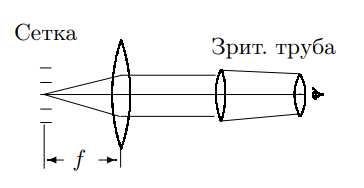
\includegraphics[width=1\linewidth]{plus_lens.PNG}
\caption{...} %% подпись к рисунку
\label{ris:experimoriginal} %% метка рисунка для ссылки на него
\end{minipage}
\hfill 
\begin{minipage}[h]{0.40\linewidth}
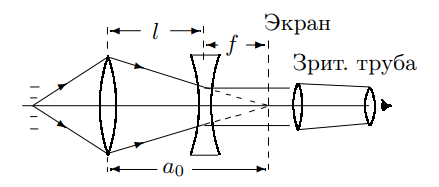
\includegraphics[width=1\linewidth]{minus_lens.PNG}
\caption{..}
\label{ris:experimcoded}
\end{minipage}
\end{center}
\end{figure}

\subsection{...}
\subsubsection{...}



\subsubsection{...}